\documentclass[titlepage]{tufte-book}

\usepackage[runall=true]{pythontex}
\setpythontexworkingdir{<outputdir>}
\usepackage{environ}
\usepackage{morewrites}
\usepackage{amsthm}
\usepackage{amsmath}
\usepackage{amssymb}
\usepackage[pdftex]{graphicx}
\usepackage{epstopdf}
\usepackage{hyperref}
\usepackage{alltt}
\usepackage{listings}
\usepackage{array}
\usepackage{extarrows}
\usepackage{setspace}
\usepackage{tikz}
\usepackage{tikz-qtree}
\usetikzlibrary{calc}
\usetikzlibrary{positioning}
\usepackage{hyperref}
\usepackage{graphviz}
\usepackage{geometry}                % See geometry.pdf to learn the layout options. There are lots.
\usepackage{bashful}
\usepackage{microtype} % Improves character and word spacing
\usepackage{caption}

\usepackage{booktabs} % Better horizontal rules in tables

\setkeys{Gin}{width=\linewidth,totalheight=\textheight,keepaspectratio} % Improves figure scaling
\graphicspath{{figures/}}

\usepackage{fancyvrb} % Allows customization of verbatim environments
\fvset{fontsize=\normalsize} % The font size of all verbatim text can be changed here

\newcounter{problem}
\newcounter{total}
\newcommand{\step}[1]{{}
\vspace{4pt} \noindent {\bf \theproblem. }#1\addtocounter{problem}{1}}

\newcommand{\cut}[1]{}

\usepackage[tikz]{bclogo}
\usepackage{tikz}
\usetikzlibrary{calc}

\lstdefinestyle{BashInputStyle}{
  language=bash,
  basicstyle=\small\ttfamily,
  numberstyle=\tiny,
  showstringspaces=false,
  numbersep=3pt,
  otherkeywords={|, ;, ', ", *,>, <, *, &, `, $},
  alsoletter={:~_},
  columns=fullflexible,
  backgroundcolor=\color{yellow!20},
  linewidth=0.93\linewidth,
  xleftmargin=0.03\linewidth,
  keywordstyle=\color{blue},
  emph={ls, cat, head, tail, more, less, sort, uniq, kill java, grep, zip, unzip, tar, wc, cp, chmod,chown},
  emphstyle=\color{black}\bfseries,
    commentstyle=\color{gray}\slshape
    }

\newcommand{\chili}{\scalebox{.04}{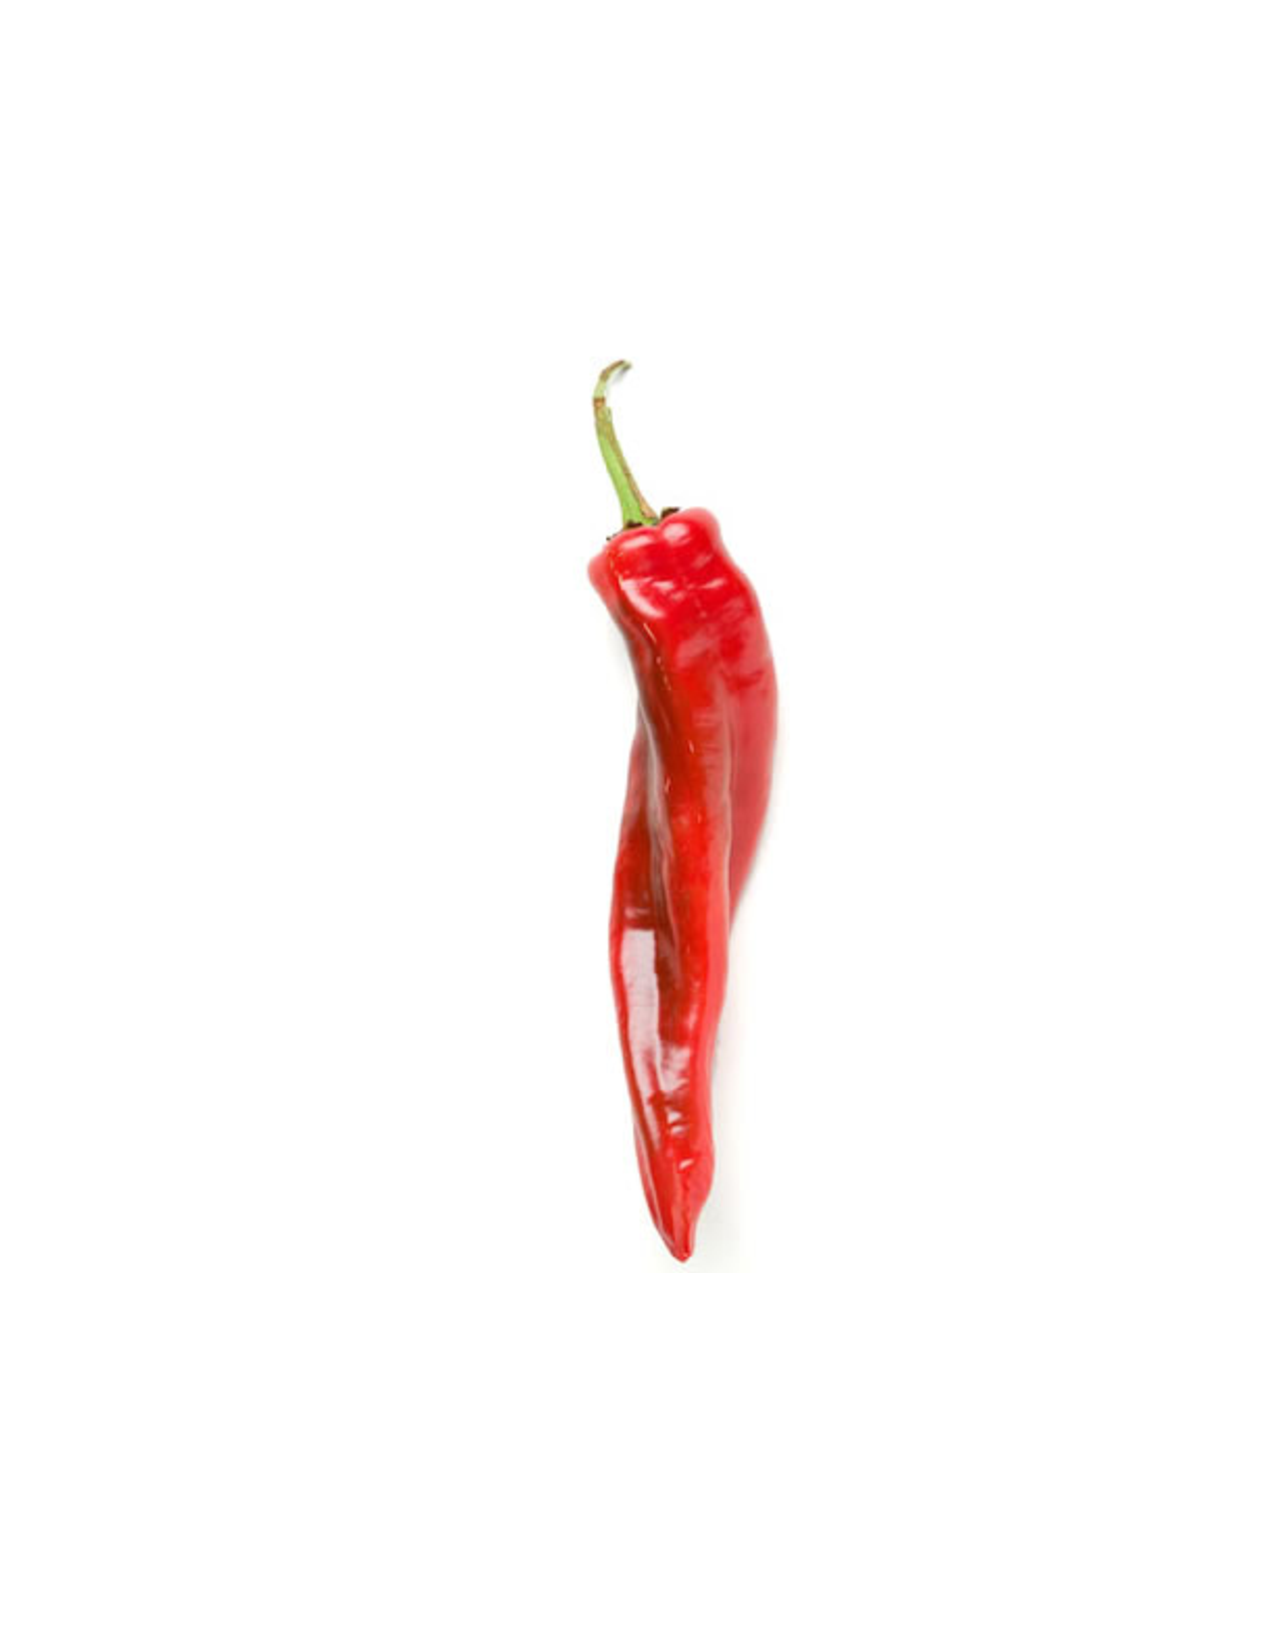
\includegraphics{figures/chili.pdf}}}
\newcommand{\chchili}{{\chili\chili}}
\newcommand{\chchchili}{{\chchili\chili}}

% The units package provides nice, non-stacked fractions and better spacing
% for units.
\usepackage{units}

% The fancyvrb package lets us customize the formatting of verbatim
% environments.  We use a slightly smaller font.
\usepackage{fancyvrb}
\fvset{fontsize=\normalsize}

% Small sections of multiple columns
\usepackage{multicol}

\hypersetup{
urlcolor=blue,
colorlinks=true
}
\usepackage[noline, procnumbered, linesnumberedhidden, boxed]{algorithm2e}

\newcommand{\openepigraph}[2]{ % This block sets up a command for printing an epigraph with 2 arguments - the quote and the author
\begin{fullwidth}
\sffamily\large
\begin{doublespace}
\noindent\allcaps{#1}\\ % The quote
\noindent\allcaps{#2} % The author
\end{doublespace}
\end{fullwidth}
}

\newcommand{\figref}[1]{Figure~\ref{#1}}
\renewcommand{\thefigure}{\arabic{figure}}

\newenvironment{callout}[1]{
\[
  \left[
      \begin{tabular}{@{\quad}m{.05\textwidth}@{\qquad}m{.75\textwidth}@{\quad}}
        \scalebox{1.5}{#1} & 
          \raggedright%
}
{
      \end{tabular}
    \right]
\]
}

\newcommand{\blankpage}{\newpage\hbox{}\thispagestyle{empty}\newpage} % Command to insert a blank page

\usepackage{makeidx} % Used to generate the index
\makeindex % Generate the index which is printed at the end of the document

\renewcommand{\maketitlepage}[0]{%
  \cleardoublepage%
  {%
  \sffamily%
  \begin{fullwidth}%
  ~
  \vspace{11.5pc}%
  \fontsize{36}{40}\selectfont\par\noindent\textcolor{darkgray}{\allcaps{\thanklesstitle}}%
  
\scalebox{.2}{
\includegraphics{figures/msan-logo}}
  \vspace{11.5pc}%
  \fontsize{12}{18}\selectfont\par\indent\textcolor{darkgray}{\allcaps{\thanklessauthor}\\
\indent{\tt parrt@cs.usfca.edu}\\
\href{http://parrt.cs.usfca.edu}{http://parrt.cs.usfca.edu}}%
  \vspace{11.5pc}%
  \fontsize{14}{16}\selectfont\par\noindent\allcaps{\thanklesspublisher}%
  \end{fullwidth}%
  }
  \thispagestyle{empty}%
  \clearpage%
}

\titlecontents{part}% FIXME
    [0em] % distance from left margin
    {\vspace{1.5\baselineskip}\begin{fullwidth}\LARGE\rmfamily\itshape} % above (global formatting of entry)
    {\contentslabel{2em}} % before w/label (label = ``II'')
    {} % before w/o label
    {\rmfamily\upshape\qquad\thecontentspage} % filler + page (leaders and page num)
    [\end{fullwidth}] % after

  \titlecontents{chapter}%
    [0em] % distance from left margin
    {\vspace{1.5\baselineskip}\begin{fullwidth}\Large\rmfamily\itshape} % above (global formatting of entry)
    {\hspace*{0em}\contentslabel{2em}} % before w/label (label = ``2'')
    {\hspace*{4em}} % before w/o label
    {\rmfamily\upshape\qquad\thecontentspage} % filler + page (leaders and page num)
    [\end{fullwidth}] % after

\titlespacing*{\chapter}{0pt}{0pt}{30pt}
\titlespacing*{\section}{0pt}{3.5ex plus 1ex minus .2ex}{2.3ex plus .2ex}
\titlespacing*{\subsection}{0pt}{3.25ex plus 1ex minus .2ex}{1.5ex plus.2ex}

\begin{document}

\chapter{Problem solving}

\setcounter{problem}{1}

\section{Some questions to get you warmed up}


{\bf Q}. You intercept an encrypted message from another student and you would like to decrypt it because you are nosy. Let's assume that the student mapped each letter of the alphabet to a different, unique letter chosen at random. How would you go about decrypting this message? Is it even possible if the mapping is truly random?

\begin{marginfigure}[-1.2in]
\begin{center}
\scalebox{.8}{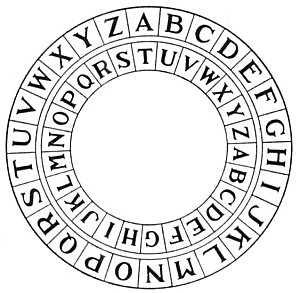
\includegraphics{figures/cipher.jpg}}
\end{center}
\caption{\tiny From {\tt http://www.sacred-texts.com/eso/sta/sta42.htm}}
\end{marginfigure}


\vspace{15mm}

\noindent {\bf Q}. Geophysicists like to explode dynamite and measure the direct and reflection waves using a ``pen on rolling paper'' device like a seismograph.  You find yourself in a remote location examining the signal from such a device and need to compute the area under the curve. The only tools you have with you are spare paper, pencil, sharp razor, ruler, and a sensitive scale. How can you get a reasonably accurate measure of the area under the seismograph curve in between two points?

\begin{marginfigure}[-1.8in]
\begin{center}
\scalebox{1}{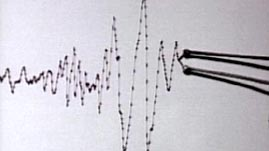
\includegraphics{figures/ess05_vid_seismograph_l.jpg}}
\end{center}
\caption{\tiny From  {\tt http://www.pbs.org/wgbh/nova/education/earth}}
\end{marginfigure}

\vspace{15mm}

\noindent {\bf Q}.  Imagine there is no symbolic solution to the area under the curve of $f(x) = \sin(x) + \frac{1}{3} \sin(3x)$ from $0$ to $\pi$. How could you estimate the area? Hint: do you like playing darts?

\begin{marginfigure}
\begin{center}
\scalebox{1}{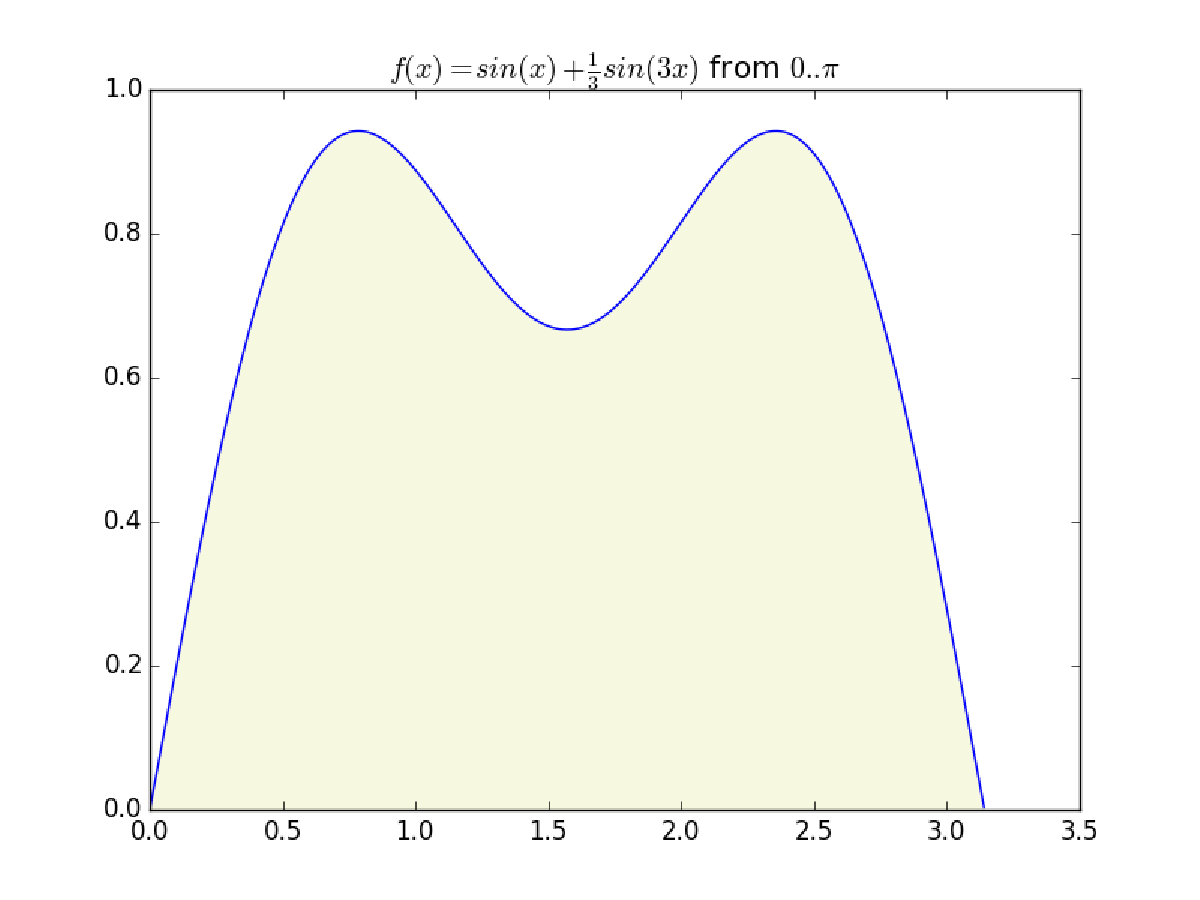
\includegraphics{figures/sin-curve.pdf}}
\end{center}
\end{marginfigure}

\vspace{20mm}

\noindent {\bf Q}.  How can you sort $N$ integers in $[0,M]$ if you can only look at each number once?

\begin{marginfigure}
\begin{center}
\scalebox{1}{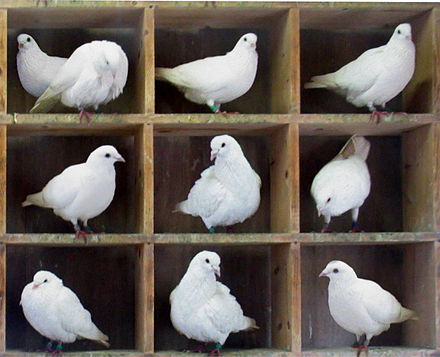
\includegraphics{figures/pigeons.jpg}}
\end{center}
\caption{\tiny From  {\tt https://en.wikipedia.org/wiki/Pigeonholing}}
\end{marginfigure}

\end{document}